% !TeX spellcheck = en_GB
\section{Building a JPA integration on top of Hibernate Search}

In this section we will start by discussing how Hibernate Search's engine (in the form of the module "hibernate-search-engine") can be used in general. Then we will work out a standalone version of this engine that is easier to work with and lastly we will show how we integrate this standalone version with JPA.

\subsection{Setting up the example project}

Before we explain how we do things in particular, we set up the example entities described in \ref{example_project} as if the original Hibernate Search would have been used. We do so by adding additional annotations to our entity-classes:

\begin{enumerate}
	\item \textbf{@Indexed}: marks the entity as an index root-type.
	\item \textbf{@DocumentId}: marks the field as the id of this entity. this is only needed if no JPA @Id can be found, but can be used to override settings.
	\item \textbf{@Field}: describes how the annotated field should be indexed. The fieldname defaults to the property name.
	\item \textbf{@IndexedEmbedded}: marks properties that point to other classes which should be included in the index. By default, all fields contained in these entities are prefixed with the property name this is placed on.
	\item \textbf{@ContainedIn}: used in entities that are embedded in other indexes. this is set on the properties that point back to the index-owning entity.
\end{enumerate}
\noindent
The resulting entities look like this:
\\
\lstset{language=java}
\lstset{moredelim=[is][\bfseries]{[*}{*]}}
\begin{lstlisting}[frame=htrbl, caption={Book.java with Hibernate Search annotations}, label={lst:book.java_2}]
@Entity
@Table(name = "Book")
[*@Indexed*]
public class Book {

	@Id
	@Column(name = "isbn")
	[*@DocumentId*]
	private String isbn;
	
	@Column(name = "title")
	[*@Field(store = Store.YES, index = Index.YES)*]
	private String title;
	
	@Column(name = "genre")
	[*@Field(store = Store.YES, index = Index.YES)*]
	private String genre;
	
	@Lob
	@Column(name = "summary")
	[*@Field(store = Store.NO, index = Index.YES)*]
	private String summary;
	
	@ManyToMany(mappedBy = "books", cascade = {
		CascadeType.MERGE,
		CascadeType.DETACH,
		CascadeType.PERSIST,
		CascadeType.REFRESH
	})
	[*@IndexedEmbedded(includeEmbeddedObjectId = true)*]
	private Set<Author> authors;
	
	//getters & setters ...
}
\end{lstlisting}

\lstset{language=java}
\lstset{moredelim=[is][\bfseries]{[*}{*]}}
\begin{lstlisting}[frame=htrbl, caption={Author.java with Hibernate Search annotations}, label={lst:author.java_2}]
@Entity
@Table(name = "Author")
public class Author {

	@Id
	@GeneratedValue(strategy = GenerationType.AUTO)
	@Column(name = "authorId")
	[*@DocumentId*]
	private Long authorId;
	
	@Column(name = "firstName")
	[*@Field(store = Store.YES, index = Index.YES)*]
	private String firstName;
	
	@Column(name = "lastName")
	[*@Field(store = Store.YES, index = Index.YES)*]
	private String lastName;
	
	@Column(name = "country")
	[*@Field(store = Store.YES, index = Index.YES)*]
	private String country;
	
	@ManyToMany(cascade = {
		CascadeType.MERGE, 
		CascadeType.DETACH, 
		CascadeType.PERSIST, 
		CascadeType.REFRESH
	})
	@JoinTable(name = "Author_Book", 
		joinColumns = 
			@JoinColumn(name = "authorFk", 
				referencedColumnName = "authorId"),
		inverseJoinColumns = 
			@JoinColumn(name = "bookFk", 
				referencedColumnName = "isbn"))
	[*@ContainedIn*]
	private Set<Book> books;
	
	//getters & setters ...
}
\end{lstlisting}
\noindent
As these annotations are defined in hibernate-search-engine, we can rely on all of them while designing the standalone version of Hibernate Search and all other modules depending on it.

\pagebreak

\subsection{Using Hibernate Search's engine} \label{using_hsearch_engine}

As already described earlier (\ref{problem_indexing_searching}), hibernate-search-engine is not intended to be used by application developers, but for other APIs to integrate with. Therefore there is no real public documentation available on how to use it and all following information had to be retrieved from tests in the hibernate-search-engine and hibernate-search-orm integration module source code.

\subsubsection{Starting the engine}
A Hibernate Search engine instance is represented by a \textbf{SearchIntegrator}. In order to obtain it, we first have to write a special configuration class that implements \textbf{org.hibernate.search.cfg.spi.SearchConfiguration}. An object of this class has then to be created and filled with all the configuration properties Hibernate Search requires. The minimum that has to be set for this to work map are the following properties:

\begin{enumerate}
	\item \textbf{hibernate.search.default.directory\_provider}: The two most common cases here are either "ram" or "filesystem". This decides where the index will be stored. A ram directory is only present in the system memory while the SearchIntegrator exists. A "filesystem" directory is persisted on the hard disk. For "filesystem" the additional property "hibernate.search.default.indexBase" has to be set to an appropriate path.
	
	\item \textbf{hibernate.search.lucene\_version}: This decides which Lucene version has to be used internally. The currently latest supported version is "4.10.4".
\end{enumerate}
\noindent
A complete list of the available settings can be found in the Hibernate Search documentation\footnote{Hibernate Search documentation, see~\cite{hibernate_search_doc}} (only some Hibernate ORM specific settings cannot be used). Our \textbf{StandaloneSearchConfiguration} (appendix listing \ref{lst:StandaloneSearchConfiguration.java}) defaults to "ram" and "4.10.4".
\\\\
Having this class in place, a \textbf{SearchIntegrator} can be obtained by a \textbf{SearchIntegratorBuilder} like this:
\\
\lstset{language=java}
\lstset{moredelim=[is][\bfseries]{[*}{*]}}
\begin{lstlisting}[frame=htrbl, caption={Starting up the engine}, label={lst:starting_up_engine.java}]
List<Class<?>> indexClasses = Arrays.asList(Book.class, Author.class);

SearchConfiguration searchConfiguration = 
	new StandaloneSearchConfiguration();
indexClasses.forEach( searchConfiguration::addClass );

//bootstrapping class for Hibernate Search
SearchIntegratorBuilder builder = new SearchIntegratorBuilder();

//we have to build an integrator here (the builder needs a 
//"base integrator" first before we can add index classes)
builder.configuration( searchConfiguration ).buildSearchIntegrator();

indexClasses.forEach( builder::addClass );

//starts the engine with all configuration properties set
SearchIntegrator searchIntegrator = builder.buildSearchIntegrator();

//use the integrator ...

//close it
searchIntegrator.close();
\end{lstlisting}

\subsubsection{Indexing, updating and deleting objects from the index}

Now that we know how a SearchIntegrator can be built, we can take a look at how we can control the index using the engine's features. 
\\\\
The engine does a lot of optimizations in the backend. This is the reason the specifics are hidden behind a \textbf{Worker} pattern. Such a worker batches operations by synchronizing upon the \textbf{org.hibernate.search.backend.TransactionContext} interface. Our implementation of this is simply called \textbf{Transaction} (appendix listing \ref{lst:Transaction.java}). The different index operations are represented by \textbf{Work} objects that contain the WorkType (INDEX, UPDATE, PURGE, etc.) and all necessary data to execute the individual task.
\\\\
Indexing objects with \textbf{WorkType.INDEX}:
\\
\lstset{language=java}
\begin{lstlisting}[frame=htrbl, caption={Indexing an object with the engine}, label={lst:indexing_object_native.java}]
Book book = ...;
Transaction tx = new Transaction();
Worker worker = searchIntegrator.getWorker();
worker.performWork( new Work( book, WorkType.INDEX ), tx );
tx.commit();
\end{lstlisting}
~\\
Updating objects with \textbf{WorkType.UPDATE}:
\\
\lstset{language=java}
\begin{lstlisting}[frame=htrbl, caption={Updating an object with the engine}, label={lst:updating_object_native.java}]
Book book = ...;
Transaction tx = new Transaction();
Worker worker = searchIntegrator.getWorker();
worker.performWork( new Work( book, WorkType.UPDATE ), tx );
tx.commit();
\end{lstlisting}
~\\
Deleting objects with \textbf{WorkType.PURGE}:
\\
\lstset{language=java}
\begin{lstlisting}[frame=htrbl, caption={Deleting an object by id with the engine}, label={lst:deleting_object_native.java}]
String isbn = ...;
Transaction tx = new Transaction();
Worker worker = searchIntegrator.getWorker();
worker.performWork( new Work( Book.class, isbn, WorkType.PURGE ), tx );
tx.commit();
\end{lstlisting}
~\\
This API doesn't have any "convenience" methods that wrap around the Transaction management if no batching is needed, nor does it have any wrapper utility for the Work object generation.

\subsubsection{Querying the index}
Querying the index is already acceptable to some extent when it comes to building the actual query. This is mainly due to the fact the query class \textbf{HSQuery} supports method chaining and that the same query builder DSL used in Hibernate Search ORM is available.
\\
\lstset{language=java}
\lstset{moredelim=[is][\bfseries]{[*}{*]}}
\begin{lstlisting}[frame=htrbl, caption={Querying the index with the engine}, label={lst:querying_natively.java}]
SearchIntegrator searchIntegrator = ...;

HSQuery query = searchIntegrator.createHSQuery();

//find information about all the entities matching a given title
[*List<EntityInfo>*] entityInfos = 
	query.luceneQuery(
			//query DSL:
			searchIntegrator.buildQueryBuilder()
				.forEntity( Book.class )
				.get()
				.keyword()
				.onField( "title" )
				.matching( "searchString" )
				.createQuery()
		).targetedEntities(
			Collections.singletonList(
				Book.class
			)
		)[*.projection(
			ProjectionConstants.ID
		)*].queryEntityInfos();
\end{lstlisting}
~\\
However, the queries don't return anything resembling the original Java objects, as this depends on what we project in the projection(...) call and is wrapped in an \textbf{EntityInfo} object. In the example above we only return the ids of the Books matching our query. We do this because when using a search index, we don't generally want to work with the actual data found in the index after the hits have been found. We want objects retrieved from the database.
\\
\lstset{language=java}
\begin{lstlisting}[frame=htrbl, caption={Extracting info from the results}, label={lst:querying_natively.java_2}]
//a JPA EntityManager
EntityManager em = ...;

//extract info from the entityInfos
for(EntityInfo entityInfo : entityInfos) {
	String isbn = (String) entityInfo.getProjection()[0];
	//retrieve an object from the database
	Book book = em.find(Book.class, isbn);
	//handle this information ...
}
\end{lstlisting}

\pagebreak

\subsection{Standalone version of Hibernate Search} \label{standalone_hibernate_search}

In \ref{using_hsearch_engine} we described how the engine can be used natively without any notion of JPA. While using the engine this way is possible, it is not feasible because some of the code is quite complicated. This is the reason, we will now discuss a standalone abstraction of this code.
\\\\
As we have seen in the examples earlier, the main class used for index control and querying are \textbf{SearchIntegrator} and \textbf{HSQuery}. In order to abstract some of the complicated logic, we now introduce two new interfaces: 

\begin{itemize}
	\item \textbf{StandaloneSearchFactory}: This interface is responsible for all index changes. Code using this abstraction doesn't have to cope with the Worker pattern, at all. This is hidden behind index/delete/update methods.
	
	\item \textbf{HSearchQuery}: While still having the same chaining methods as HSQuery, we retrieve results from the index in a different manner now. Instead of manually having to extract the ID out of the EntityInfos, this interface retrieves the actual data needed by the calling code with the help of the \textbf{EntityProvider} interface which wraps the access to the database. The specifics of the EntityProvider are still use-case specific as the examples later in this chapter will show.
\end{itemize}
\noindent
The following diagram shows the rough architecture of our new standalone. Note that we are using a specialization of \textbf{SearchIntegrator} - namely \textbf{ExtendedSearchIntegrator} - which allows us to have more sophisticated features.

\begin{figure}[ht]
	\centering
	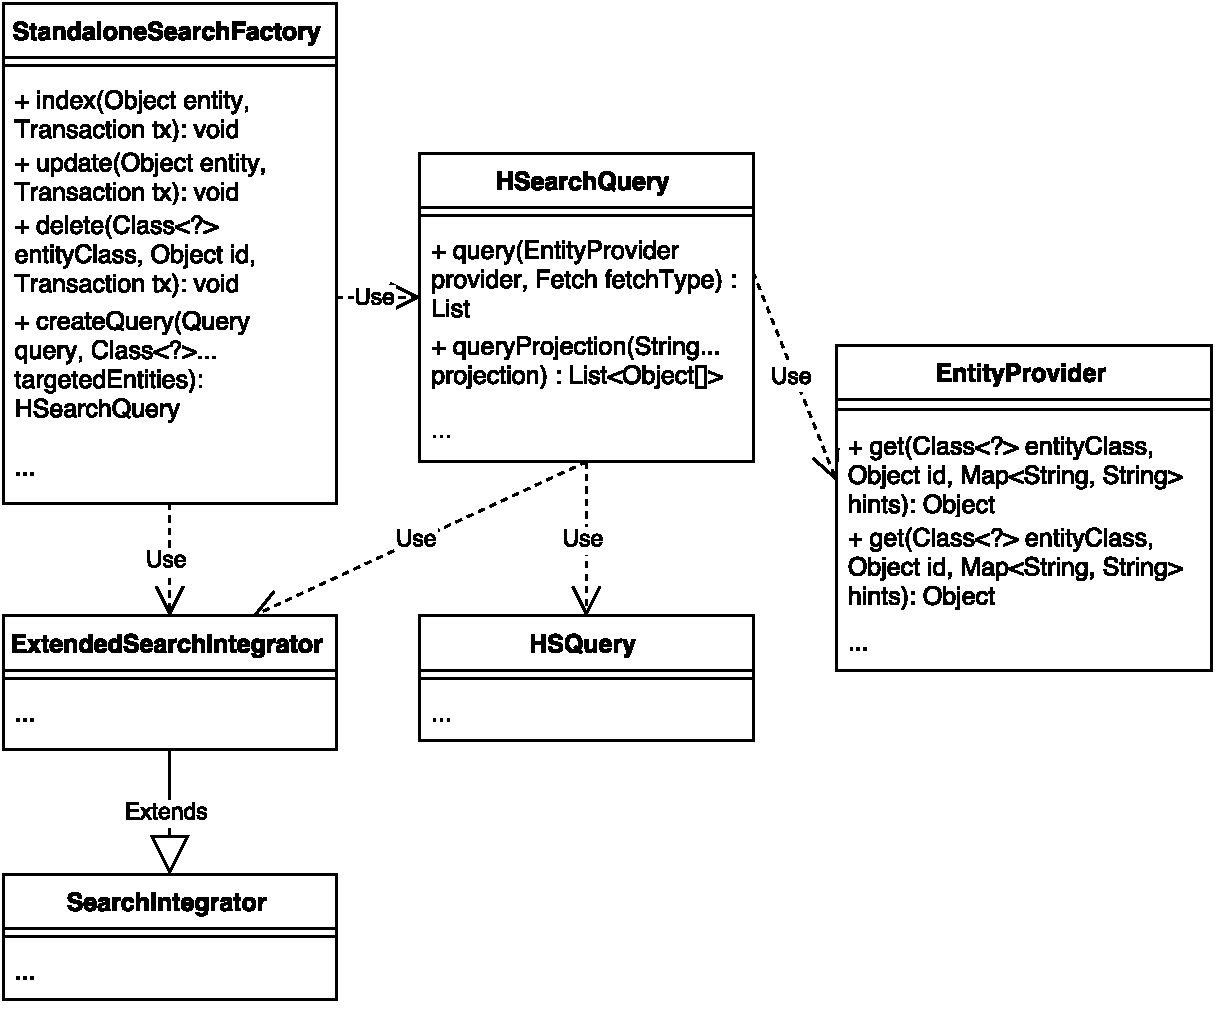
\includegraphics[scale=0.6]{images/standalone_min_architecture.pdf}
	\caption{Rough architecture of the standalone (important parts)}
	\label{standalone_min_architecture}
\end{figure}

\subsubsection{Starting the standalone}

The startup process of the standalone doesn't differ much from manually using the engine in terms of configuration as we still have to use the SearchConfiguration interface. The only different thing is how we build the StandaloneSearchFactory. This is done with a \textbf{StandaloneSearchFactoryFactory}, so the code using it doesn't have to handle the creation of an the actual implementation object.
\\
\lstset{language=java}
\lstset{moredelim=[is][\bfseries]{[*}{*]}}
\begin{lstlisting}[frame=htrbl, caption={Starting up the standalone}, label={lst:using_standalone.java}]
List<Class<?>> indexClasses = Arrays.asList(Book.class, Author.class);

SearchConfiguration searchConfiguration = 
		new StandaloneSearchConfiguration();
indexClasses.forEach( searchConfiguration::addClass );

StandaloneSearchFactory searchFactory = 
		StandaloneSearchFactoryFactory.
				createSearchFactory(
					searchConfiguration,
					indexClasses
				);
				
//use the searchfactory ...

//close it
searchFactory.close();
\end{lstlisting}

\subsubsection{Indexing, updating and deleting objects from the index}

With our standalone version, basic index control becomes more streamlined as we don't have to work with  SearchIntegrator's Worker pattern anymore.
\\
\lstset{language=java}
\begin{lstlisting}[frame=htrbl, caption={Indexing an object with the standalone}, label={lst:indexing_object_native.java}]
Book book = ...;
Transaction tx = new Transaction();
searchFactory.index(book, tx);
tx.commit();
\end{lstlisting}

\lstset{language=java}
\begin{lstlisting}[frame=htrbl, caption={Updating an object with the standalone}, label={lst:updating_object_native.java}]
Book book = ...;
Transaction tx = new Transaction();
searchFactory.update(book, tx);
tx.commit();
\end{lstlisting}

\lstset{language=java}
\begin{lstlisting}[frame=htrbl, caption={Deleting an object by id with the standalone}, label={lst:deleting_object_native.java}]
Transaction tx = new Transaction();
String isbn = ...;
searchFactory.delete(Book.class, isbn, tx);
tx.commit();
\end{lstlisting}

\subsubsection{Querying the index}
The biggest change in the standalone version is probably how the index is queried. We don't have to work with EntityInfos anymore as we introduce the \textbf{EntityProvider} interface. This interface hosts one method that is to be used for batch fetching (Fetch.BATCH) and one for single fetching (FETCH.FIND\_BY\_ID).
\\\\
A good default implementation delegating the database access to a JPA EntityManager is our \textbf{BasicEntityProvider} (\ref{lst:BasicEntityProvider.java}). Besides taking a EntityManager in its constructor, the class also needs a Map<Class<?>, String> containing the id properties of the entities. While we leave the construction of this map out in the following example for the sake of simplicity, the code for this can be found in the listings (\ref{lst:idProperties.java}). After its creation this map can then be stored in a central place and be reused.
\\
\lstset{language=java}
\begin{lstlisting}[frame=htrbl, caption={Querying the index with the standalone}, label={lst:querying_natively.java}]
StandaloneSearchFactory searchFactory = ...;

EntityManager em = ...;
Map<Class<?>, String> idProperties = ...;

EntityProvider entityProvider = new BasicEntityProvider(em, idProperties);

List<Book> = searchFactory.createQuery(searchFactory.buildQueryBuilder()
				.forEntity(Book.class)
				.get()
				.keyword()
				.onField("title")
				.matching("searchString")
				.createQuery(), Book.class
			).query(
				entityProvider,
				Fetch.BATCH
			);
\end{lstlisting}

\pagebreak

\subsection{Standalone integration with JPA interfaces}
After simplifying the access to Hibernate Search's engine we will work out an integration with JPA interfaces next. Since we started with the premise of not wanting to "reinvent the wheel" by writing everything from scratch - which was one of the reasons why we chose to use Hibernate Search's engine in the first place - we will try to build an integration as similar to the JPA interfaces of Hibernate Search ORM as possible.
\\\\
Before we can go into detail about how we build our integration, we have to discuss the general architecture first. We will go over how the Hibernate Search ORM integration with JPA interfaces works and then take a look at what has to be changed in order to work with any JPA implementor.

\subsubsection{Architecture of Hibernate Search ORM}

Hibernate Search ORM integrates with the JPA API by extending the interfaces  javax.persistence.EntityManager and javax.persistence.Query and adding new functionality to the fulltext search versions of these interfaces: \textbf{FullTextEntityManager} and \textbf{FullTextQuery}. The following figure shows a rough overview of this. Note that this only contains only the methods relevant for the following inspections.
\\
\begin{figure}[ht]
	\centering
	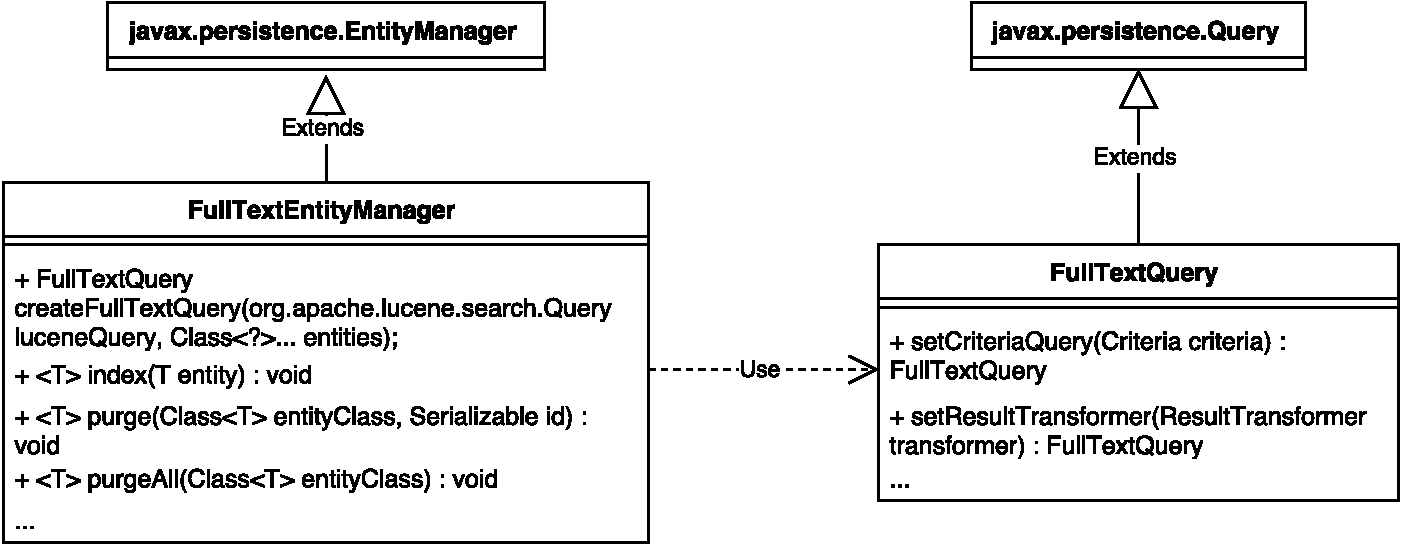
\includegraphics[scale=0.6]{images/hibernate_search_jpa_integration_original.pdf}
	\caption{The main JPA interfaces of Hibernate Search ORM}
	\label{hibernate_search_jpa_integration_original}
\end{figure}

\paragraph{Starting}
As Hibernate Search ORM is tightly coupled with Hibernate ORM it is automatically started if found on the classpath and the persistence.xml contains the following:
\\
\lstset{language=java}
\begin{lstlisting}[frame=htrbl, caption={Additions to persistence.xml with Hibernate Search ORM}, label={lst:hibernate_search_persistence.xml}]
...
<property name="hibernate.search.default.directory_provider"
value="filesystem"/>
<property name="hibernate.search.default.indexBase"
value="/path/to/indexes"/>
...
\end{lstlisting}
\noindent
This means that there exists no real code entry point as Hibernate Search is fully integrated into the Hibernate ORM/OGM lifecycle. FullTextEntityManagers can therefore be obtained with:
\\
\lstset{language=java}
\begin{lstlisting}[frame=htrbl, caption={Obtaining a FullTextEntityManager with Hibernate Search ORM}, label={lst:indexing_object_hsearch_orm_jpa.java}]
EntityManager em = ...;
FullTextEntityManager fem = Search.getFullTextEntityManager(em);
\end{lstlisting}
All of FullTextEntityManagers operations are controlled by the same transactions the original Hibernate EntityManager is using. This is the reason we will not have any Transaction related code in the following paragraphs.

\paragraph{Indexing, updating and deleting objects from the index}
The index operations are all straightforward and are similar to what we designed our Standalone integration in \ref{standalone_hibernate_search} to work like apart from minor naming differences. 
\\\\
Hibernate Search ORM doesn't differentiate between indexing and updating.
\\
\lstset{language=java}
\begin{lstlisting}[frame=htrbl, caption={Indexing/Updating an object with Hibernate Search ORM}, label={lst:indexing_object_hsearch_orm_jpa.java}]
FullTextEntityManager fem = ...;
Book book = ...;
fem.index(book);
\end{lstlisting}
\noindent
Deleting objects from the index is called purging. This is probably due to not wanting to confuse it with JPAs delete(...).
\\
\lstset{language=java}
\begin{lstlisting}[frame=htrbl, caption={Deleting an object by id with Hibernate Search ORM}, label={lst:deleting_object_hsearch_orm_jpa.java}]
FullTextEntityManager fem = ...;
String isbn = ...;
fem.purge(Book.class, isbn);
\end{lstlisting}

\paragraph{Querying the index}
\lstset{language=java}
\begin{lstlisting}[frame=htrbl, caption={Querying with Hibernate Search ORM}, label={lst:querying_hsearch_orm.java_1}]
EntityManager em = ...;
FullTextEntityManager fem = Search.getFullTextEntityManager(em);

FullTextQuery fullTextQuery = fem.createFullTextQuery(
	searchFactory.buildQueryBuilder()
		.forEntity(Book.class)
		.get()
		.keyword()
		.onField("title")
		.matching("searchString")
		.createQuery(), 
	Book.class);
	
List<Book> books = (List<Book>) fullTextQuery.getResultList();
\end{lstlisting}

\begin{figure}[ht]
	\centering
	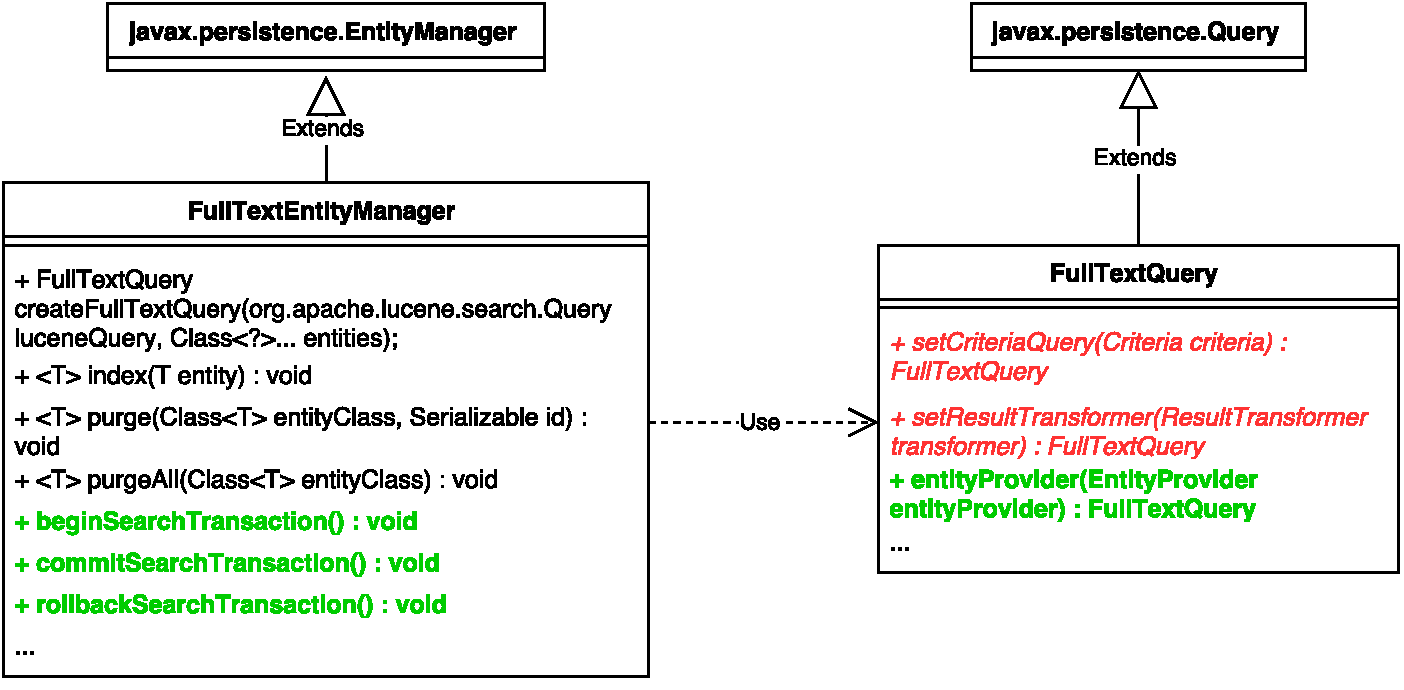
\includegraphics[scale=0.6]{images/hibernate_search_jpa_integration_with_differences.pdf}
	\caption{The main JPA interfaces of Hibernate Search}
	\label{hibernate_search_jpa_integration_with_differences}
\end{figure}

\paragraph{Index rebuilds}

\subsubsection{Architecture of the generic version}

\textcolor{red}{zusätzliche annotations, restriktionen!}

\paragraph{Starting}

\paragraph{Indexing, updating and deleting objects from the index}

\paragraph{Querying the index}

\paragraph{Index rebuilds}

\subsubsection{Implementation Details}

-> SubClassSupportInstanceInitializer, MassIndexer, Transaction Management





-> 


\pagebreak